\documentclass[11pt]{article}

%defines page size and margins
\usepackage{geometry}
\geometry{
  letterpaper,
  left=1in,
  right=1in,
  top=1in,
  bottom=1in,
}

%Sets spacing for entire document
\usepackage{setspace}
\singlespacing

%Package for reducing space in between list items
\usepackage{enumitem}

%Links
\usepackage{hyperref}

%Math symbols
\usepackage{gensymb}

%For floating images
\usepackage{float}

%better tables
\usepackage{multirow}
\usepackage{array}

\usepackage{longtable}

%Used for adjusting images
\usepackage[export]{adjustbox}

%Image path
\usepackage{graphicx}
\usepackage{animate}

\begin{document}

{\Large\noindent Brett Levenson, Andy Poulos, Rishabh Shah, John Stefan

\noindent October 2, 2017

\noindent Lab 2 \\}

\section*{Exercise One:}

\begin{figure}[H]
	\centering
	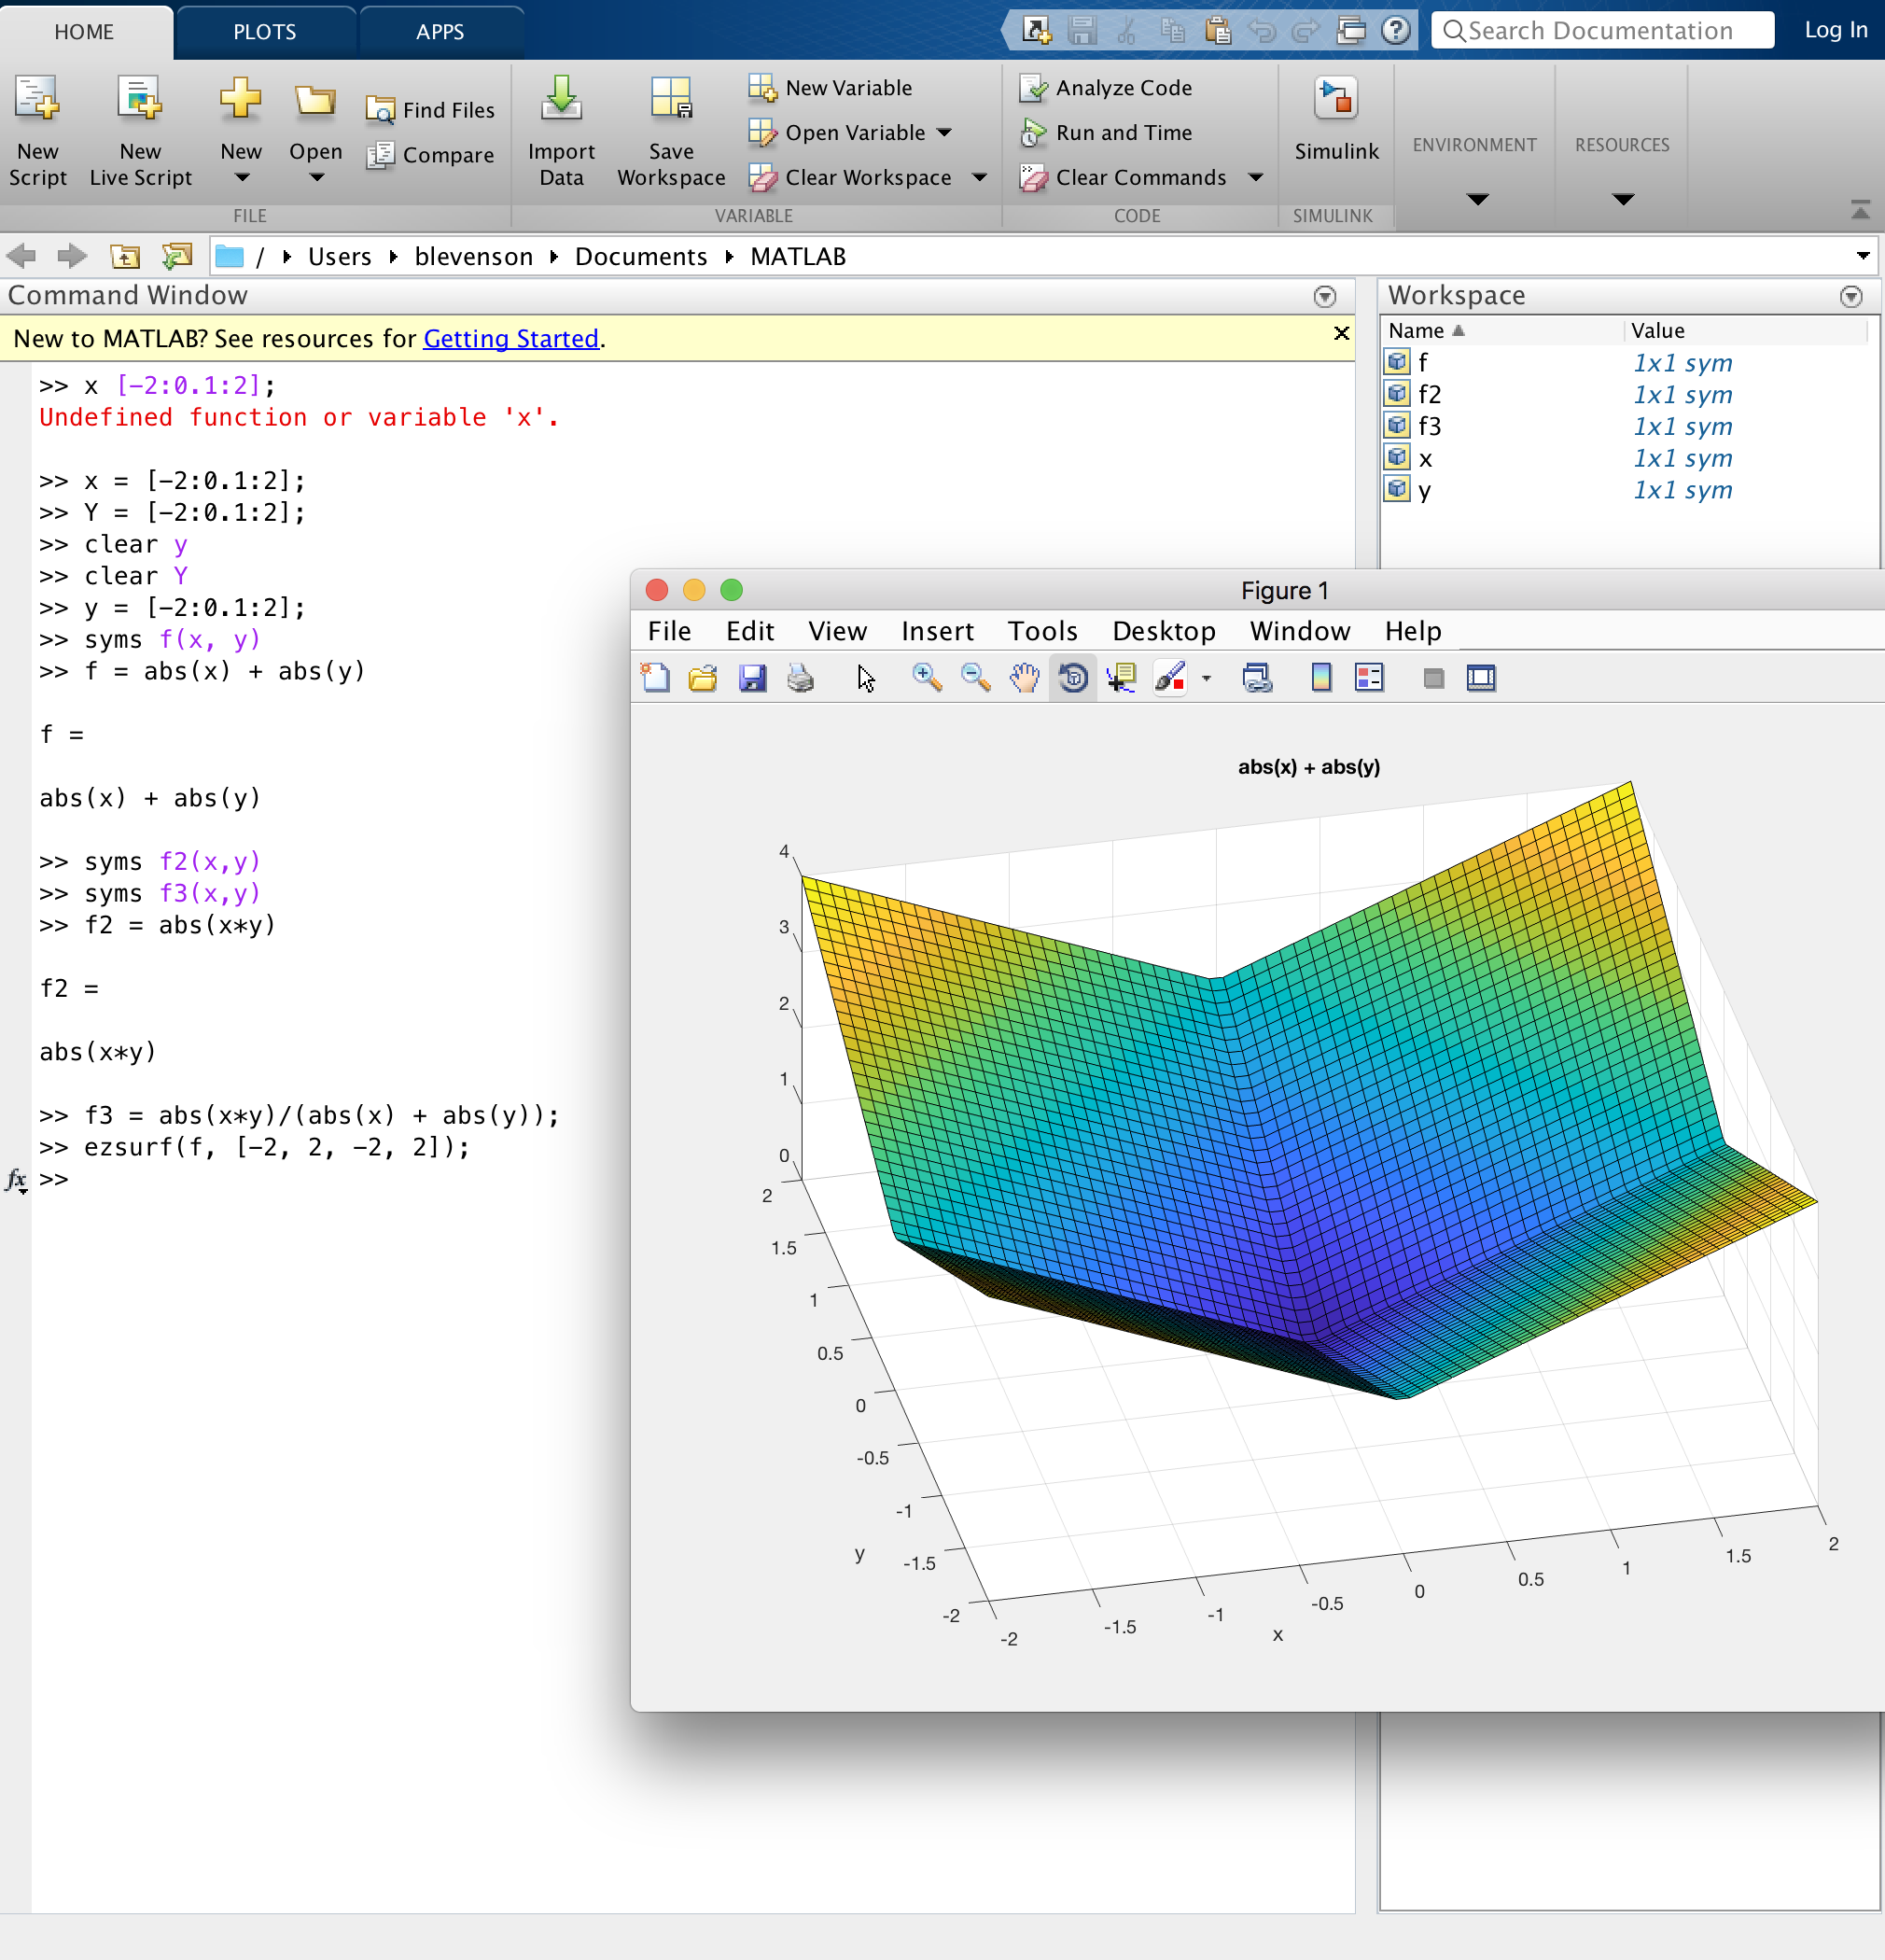
\includegraphics[width=\textwidth]{PartOne_1}
\end{figure}

\begin{figure}[H]
	\centering
	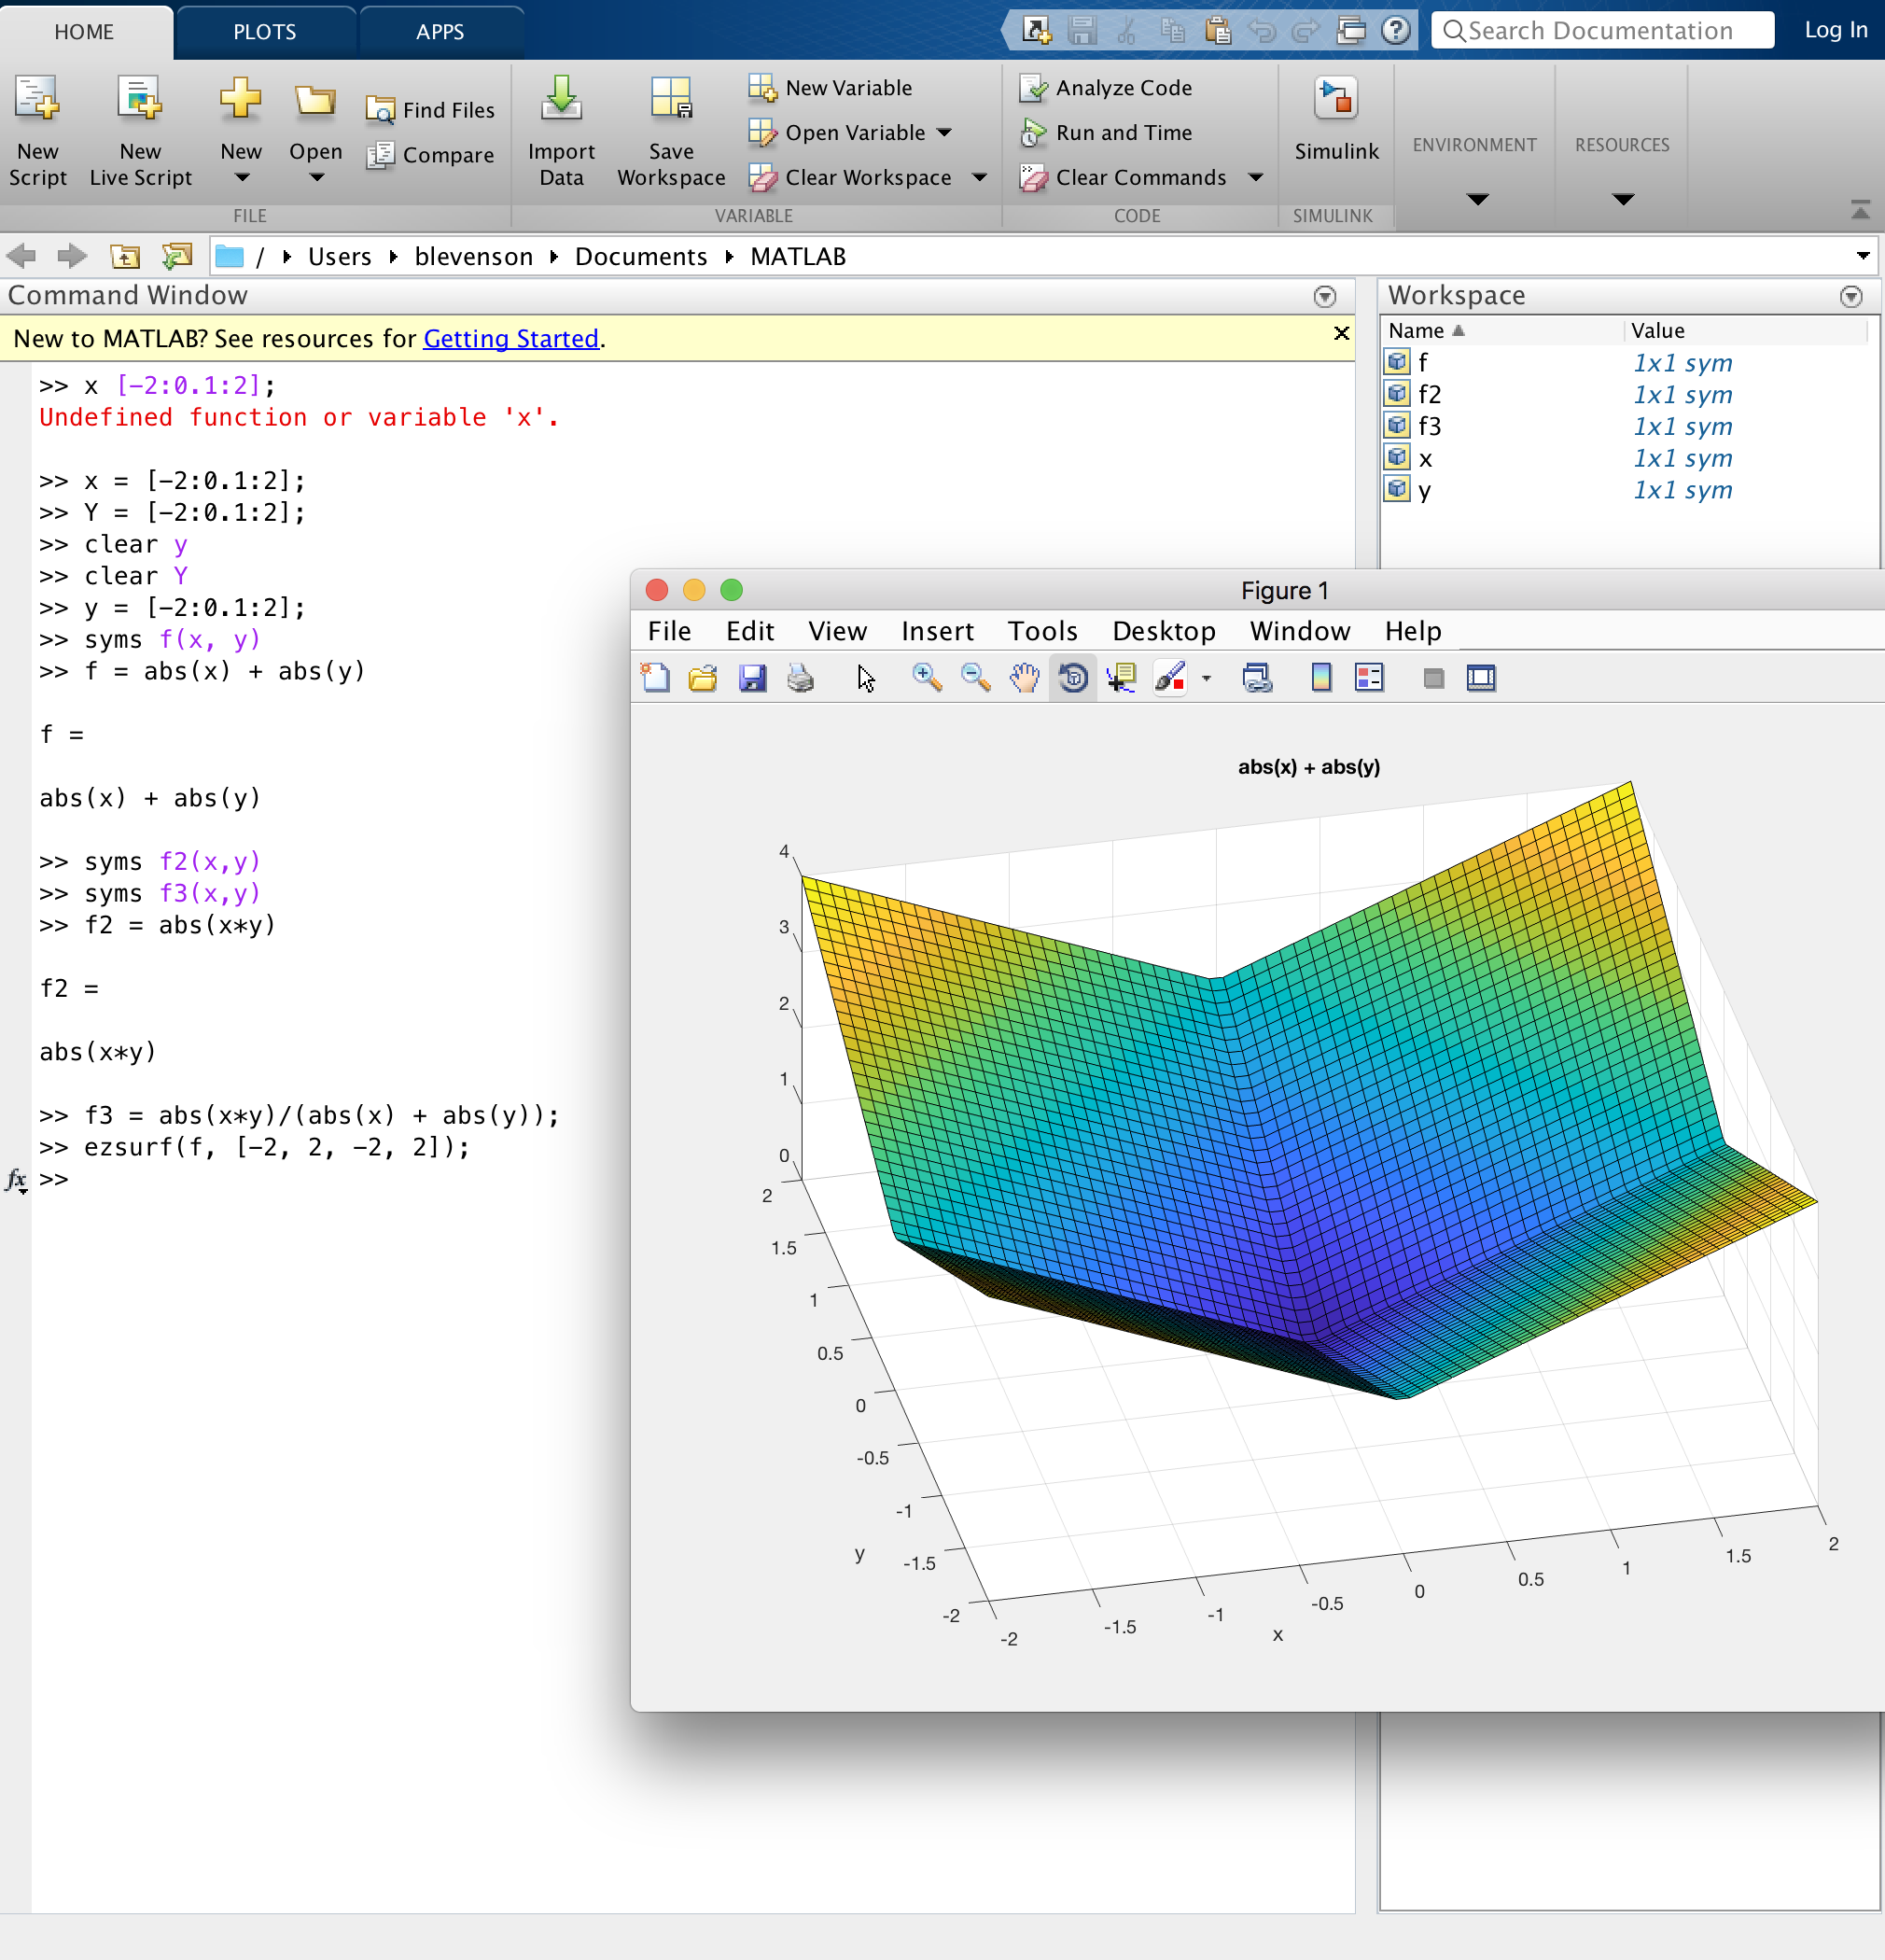
\includegraphics[width=\textwidth]{PartOne_1}
\end{figure}

\begin{figure}[H]
	\centering
	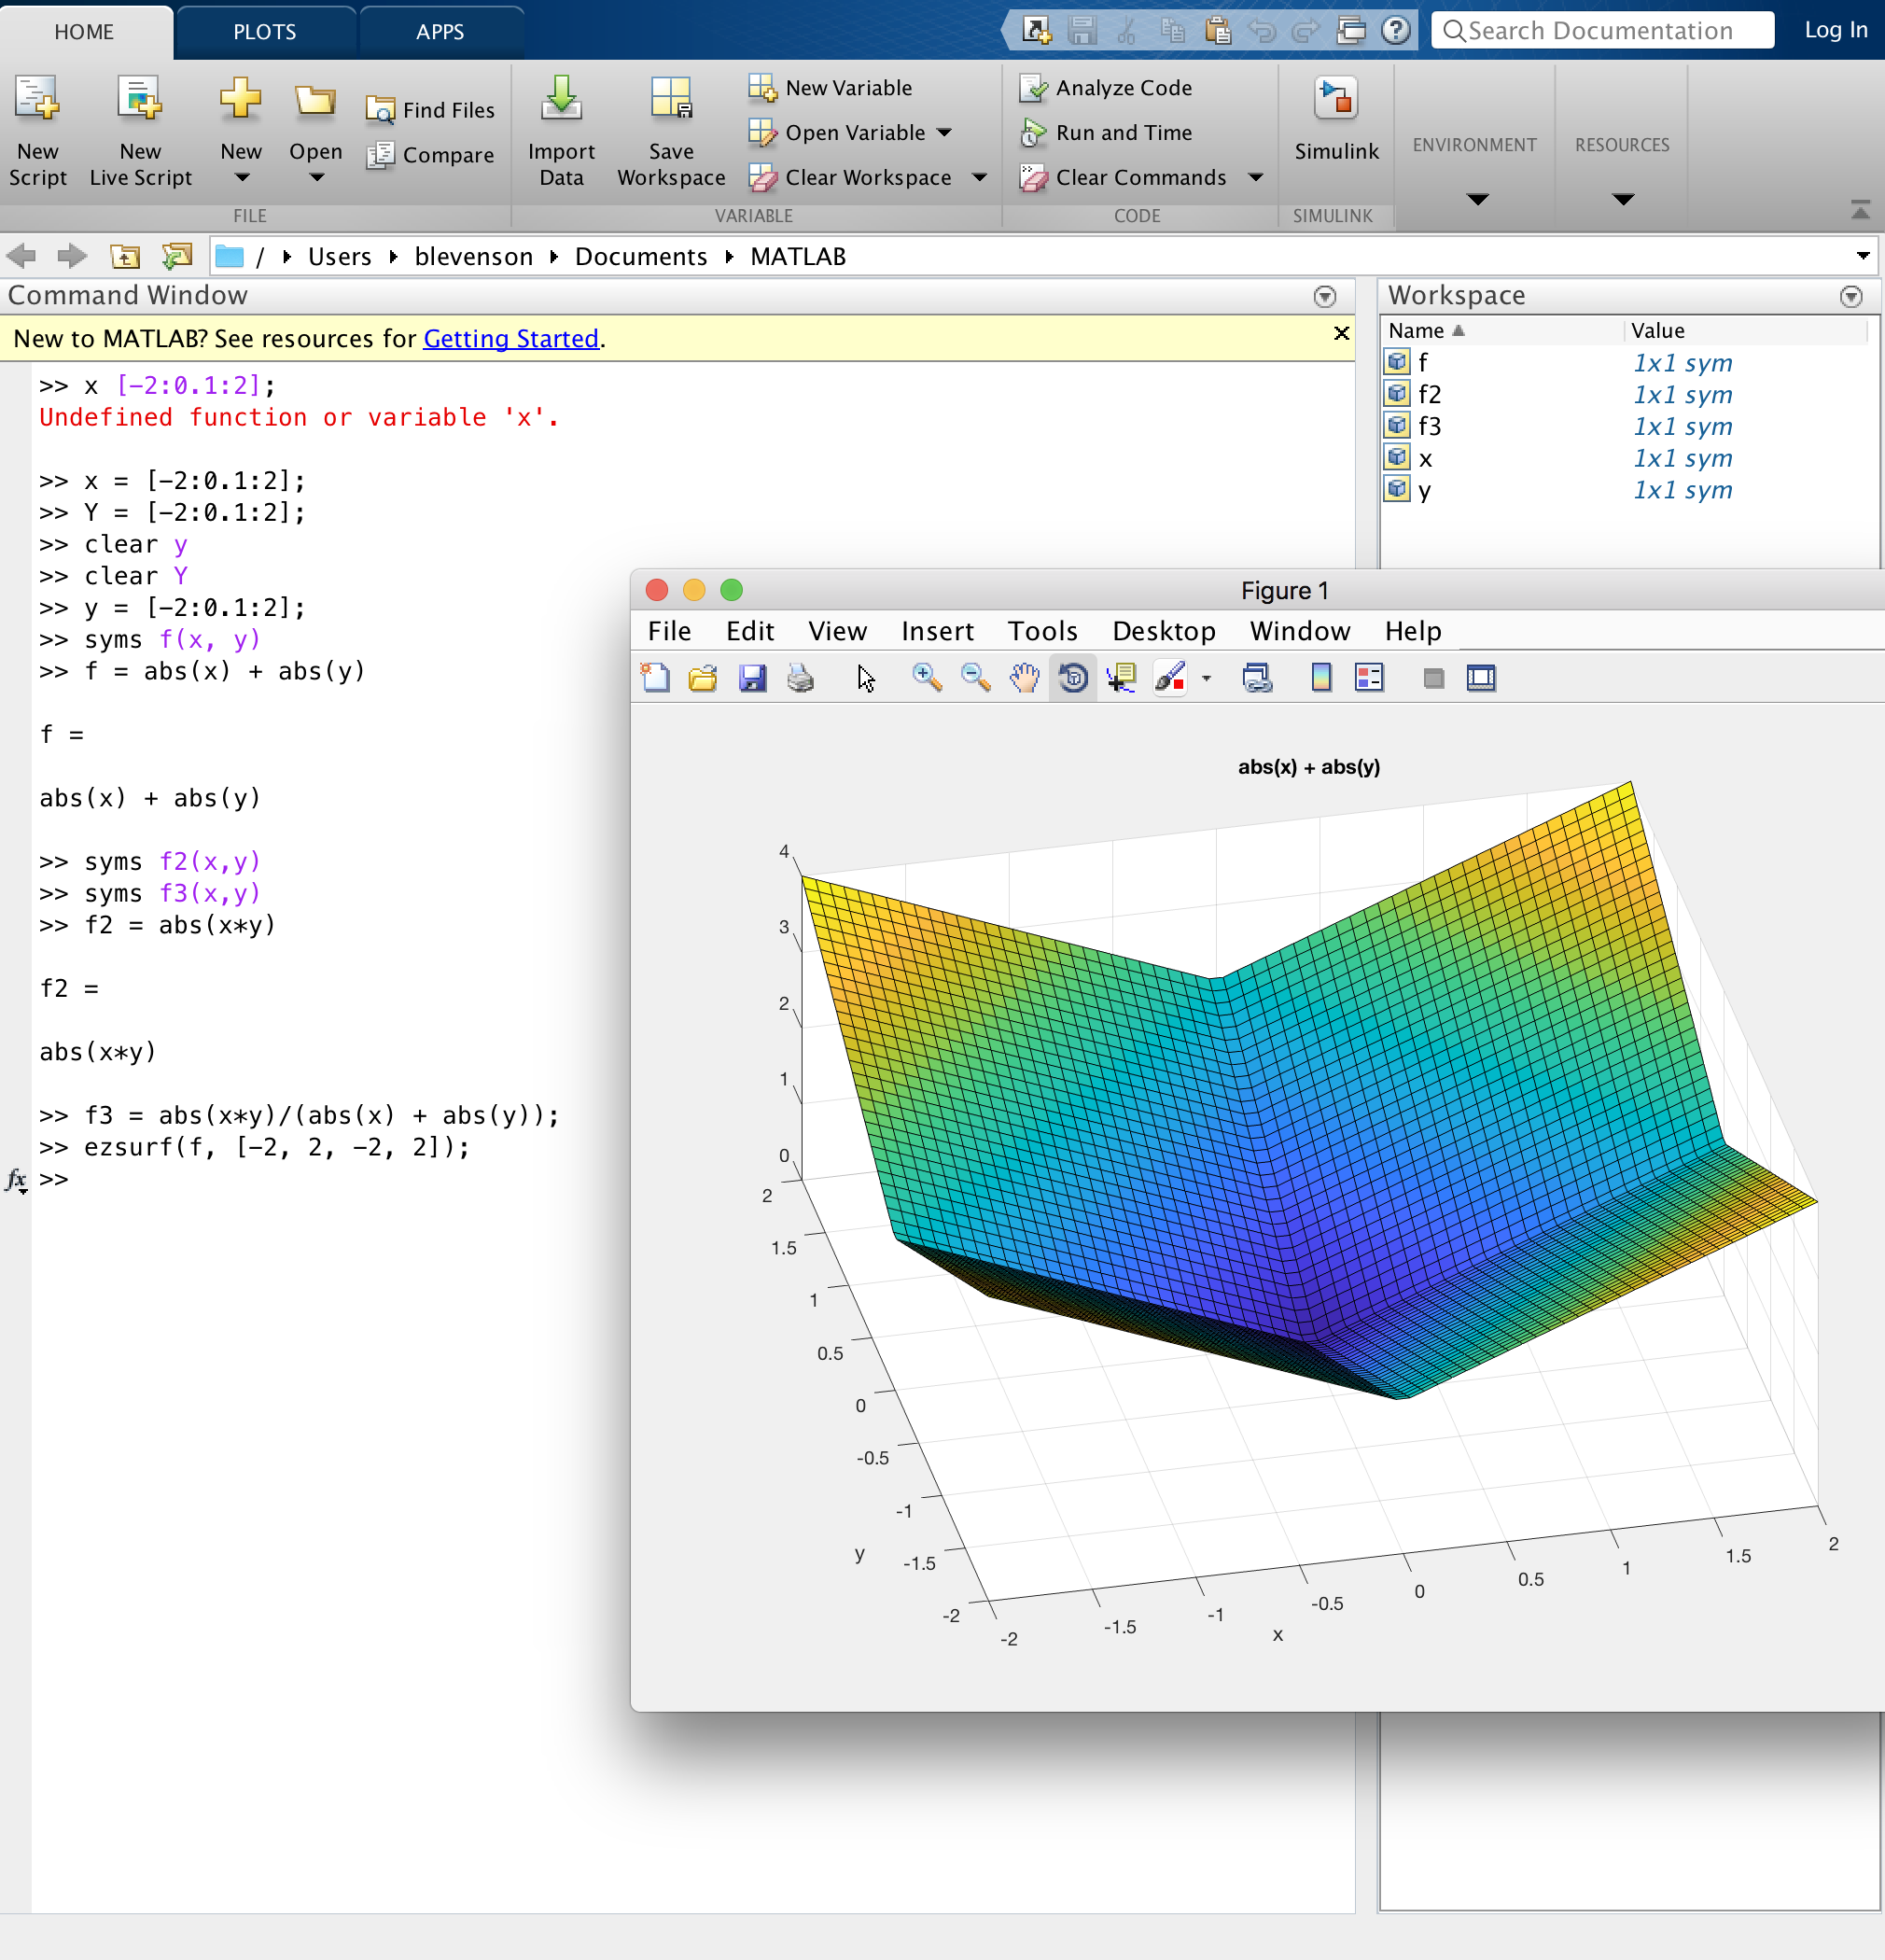
\includegraphics[width=\textwidth]{PartOne_1}
\end{figure}

\section*{Exercise Two:}
\begin{figure}[H]
	\centering
	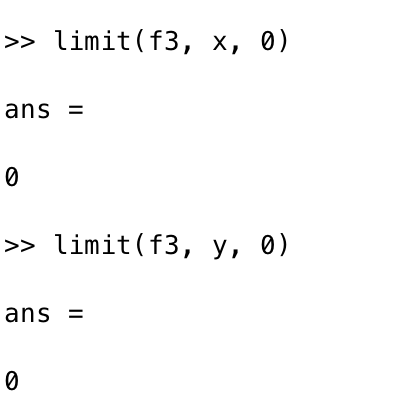
\includegraphics[width=\textwidth]{PartTwo}
	\caption{$f_3 (0,0)= 0$ will make the function $f_3$ continuous at the organ. This works because the limit as you approach this point along the $x$ axis, where the $y$ value is held to zero, the limit approaches $z = 0$.  By the same token, as you approach along the y-axis, where the $x$ value is kept at zero, it too approaches $z = 0$. While this does not show that the limit works for all possible ways of approaching the point $(0, 0)$, it is enough for us to assume $f_3 (0, 0) = 0$.}
\end{figure}

\section*{Exercise Three:}
\begin{figure}[H]
	\centering
	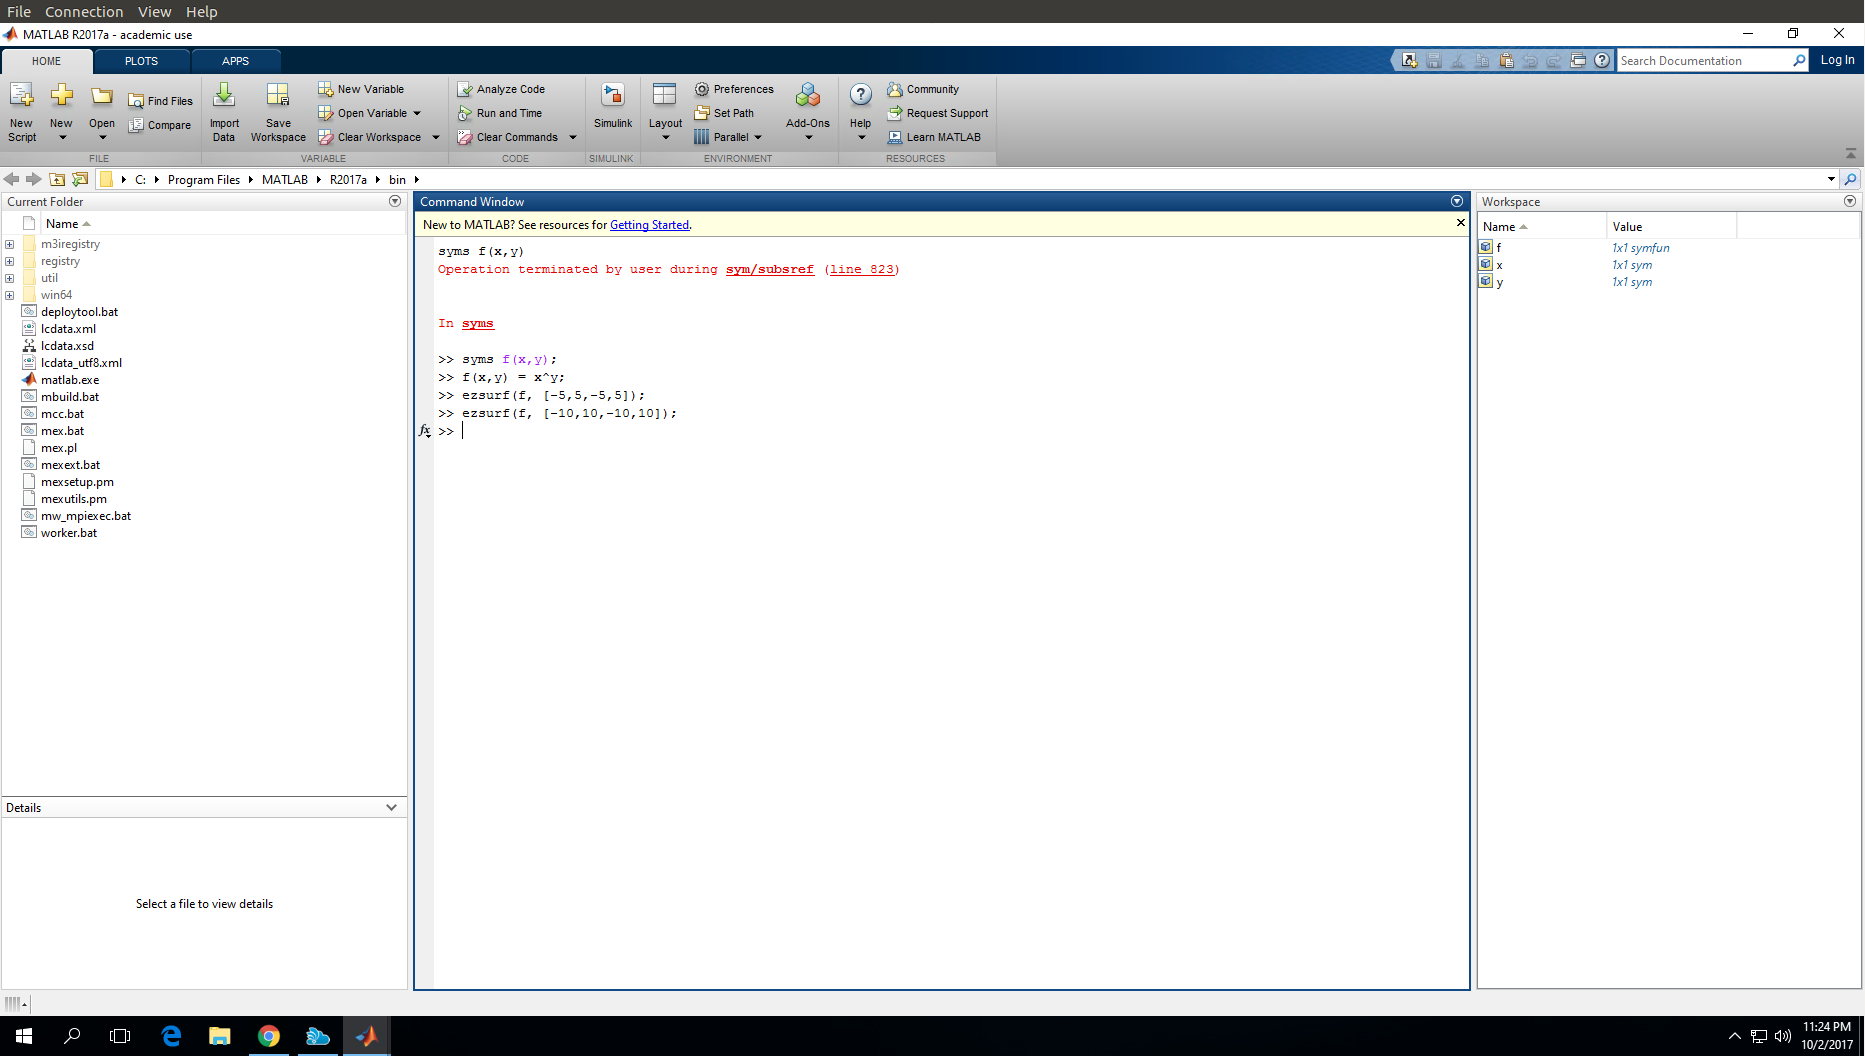
\includegraphics[width=\textwidth]{PartThree_1.png}
\end{figure}

\begin{figure}[H]
	\centering
	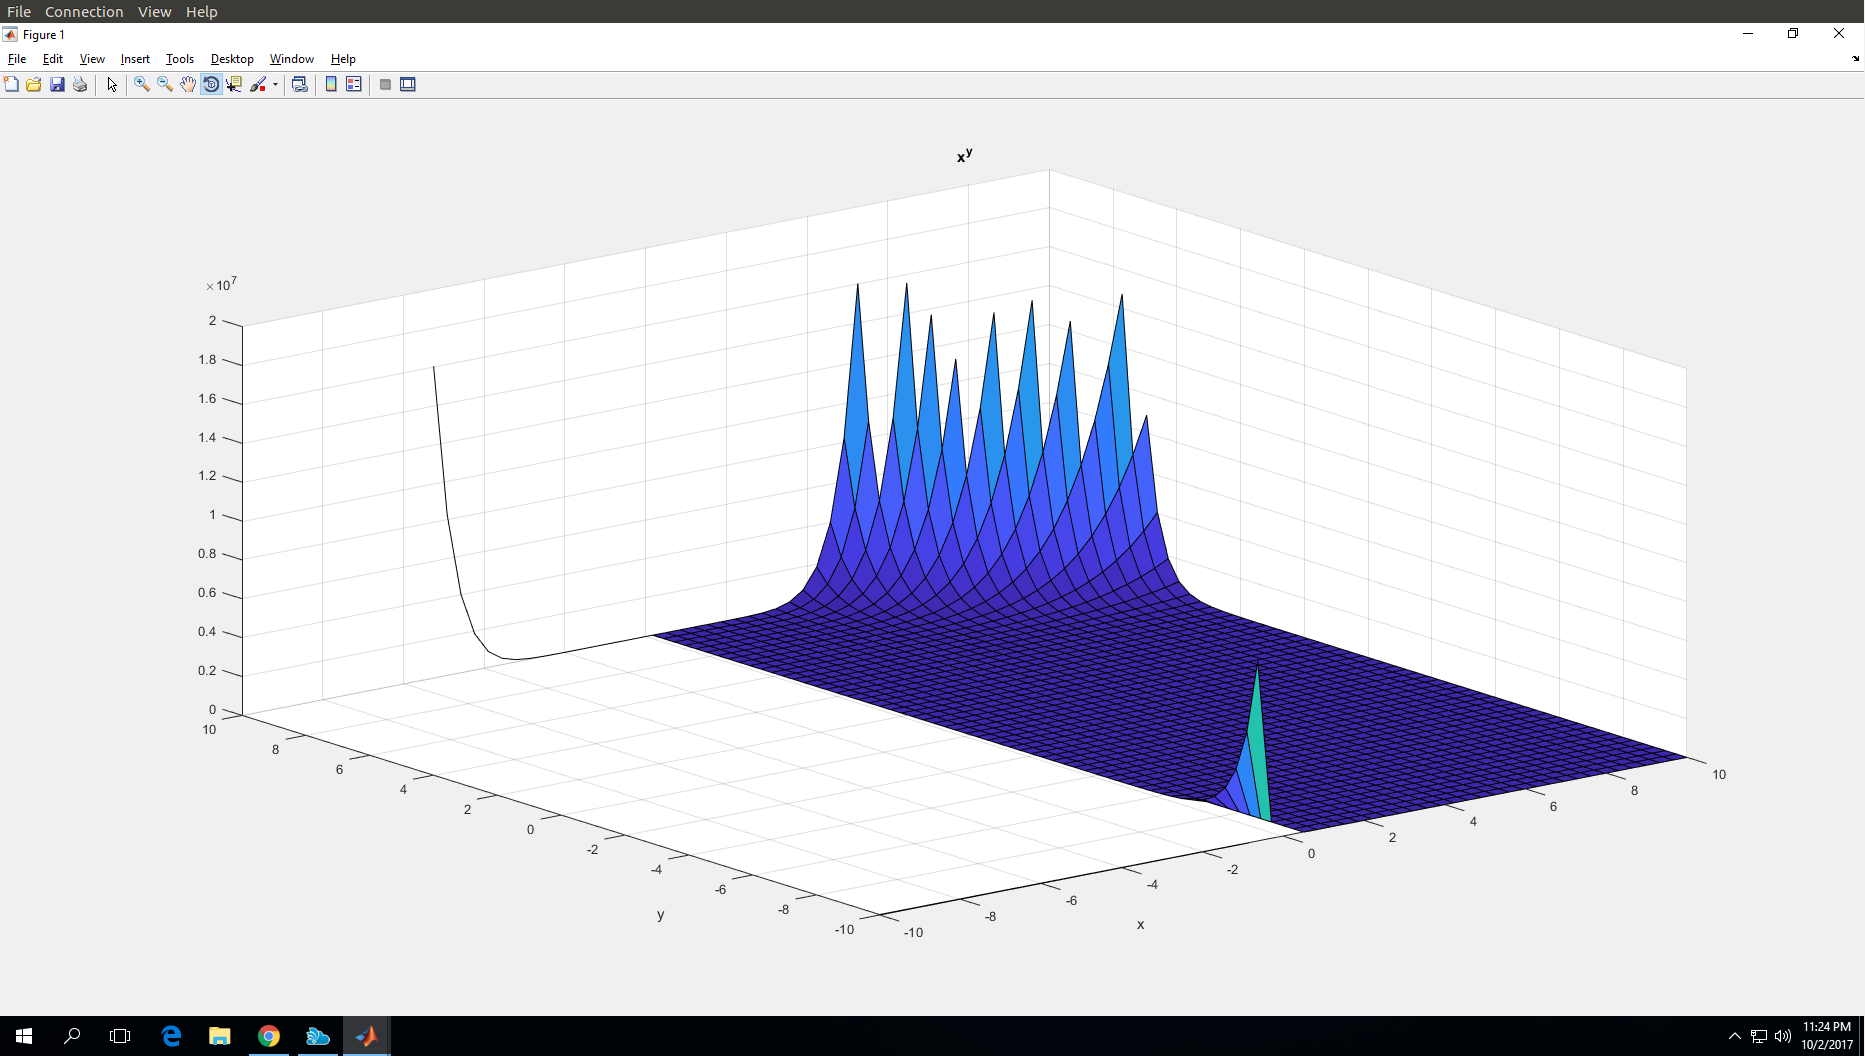
\includegraphics[width=\textwidth]{PartThree_2.png}
\end{figure}

I do not think it is possible to assign a value to $f(0,0)$ to make $f$ continuous because there are no values for which $f$ will be continuous.

\section*{Exercise Four:}
\begin{figure}[H]
	\centering
	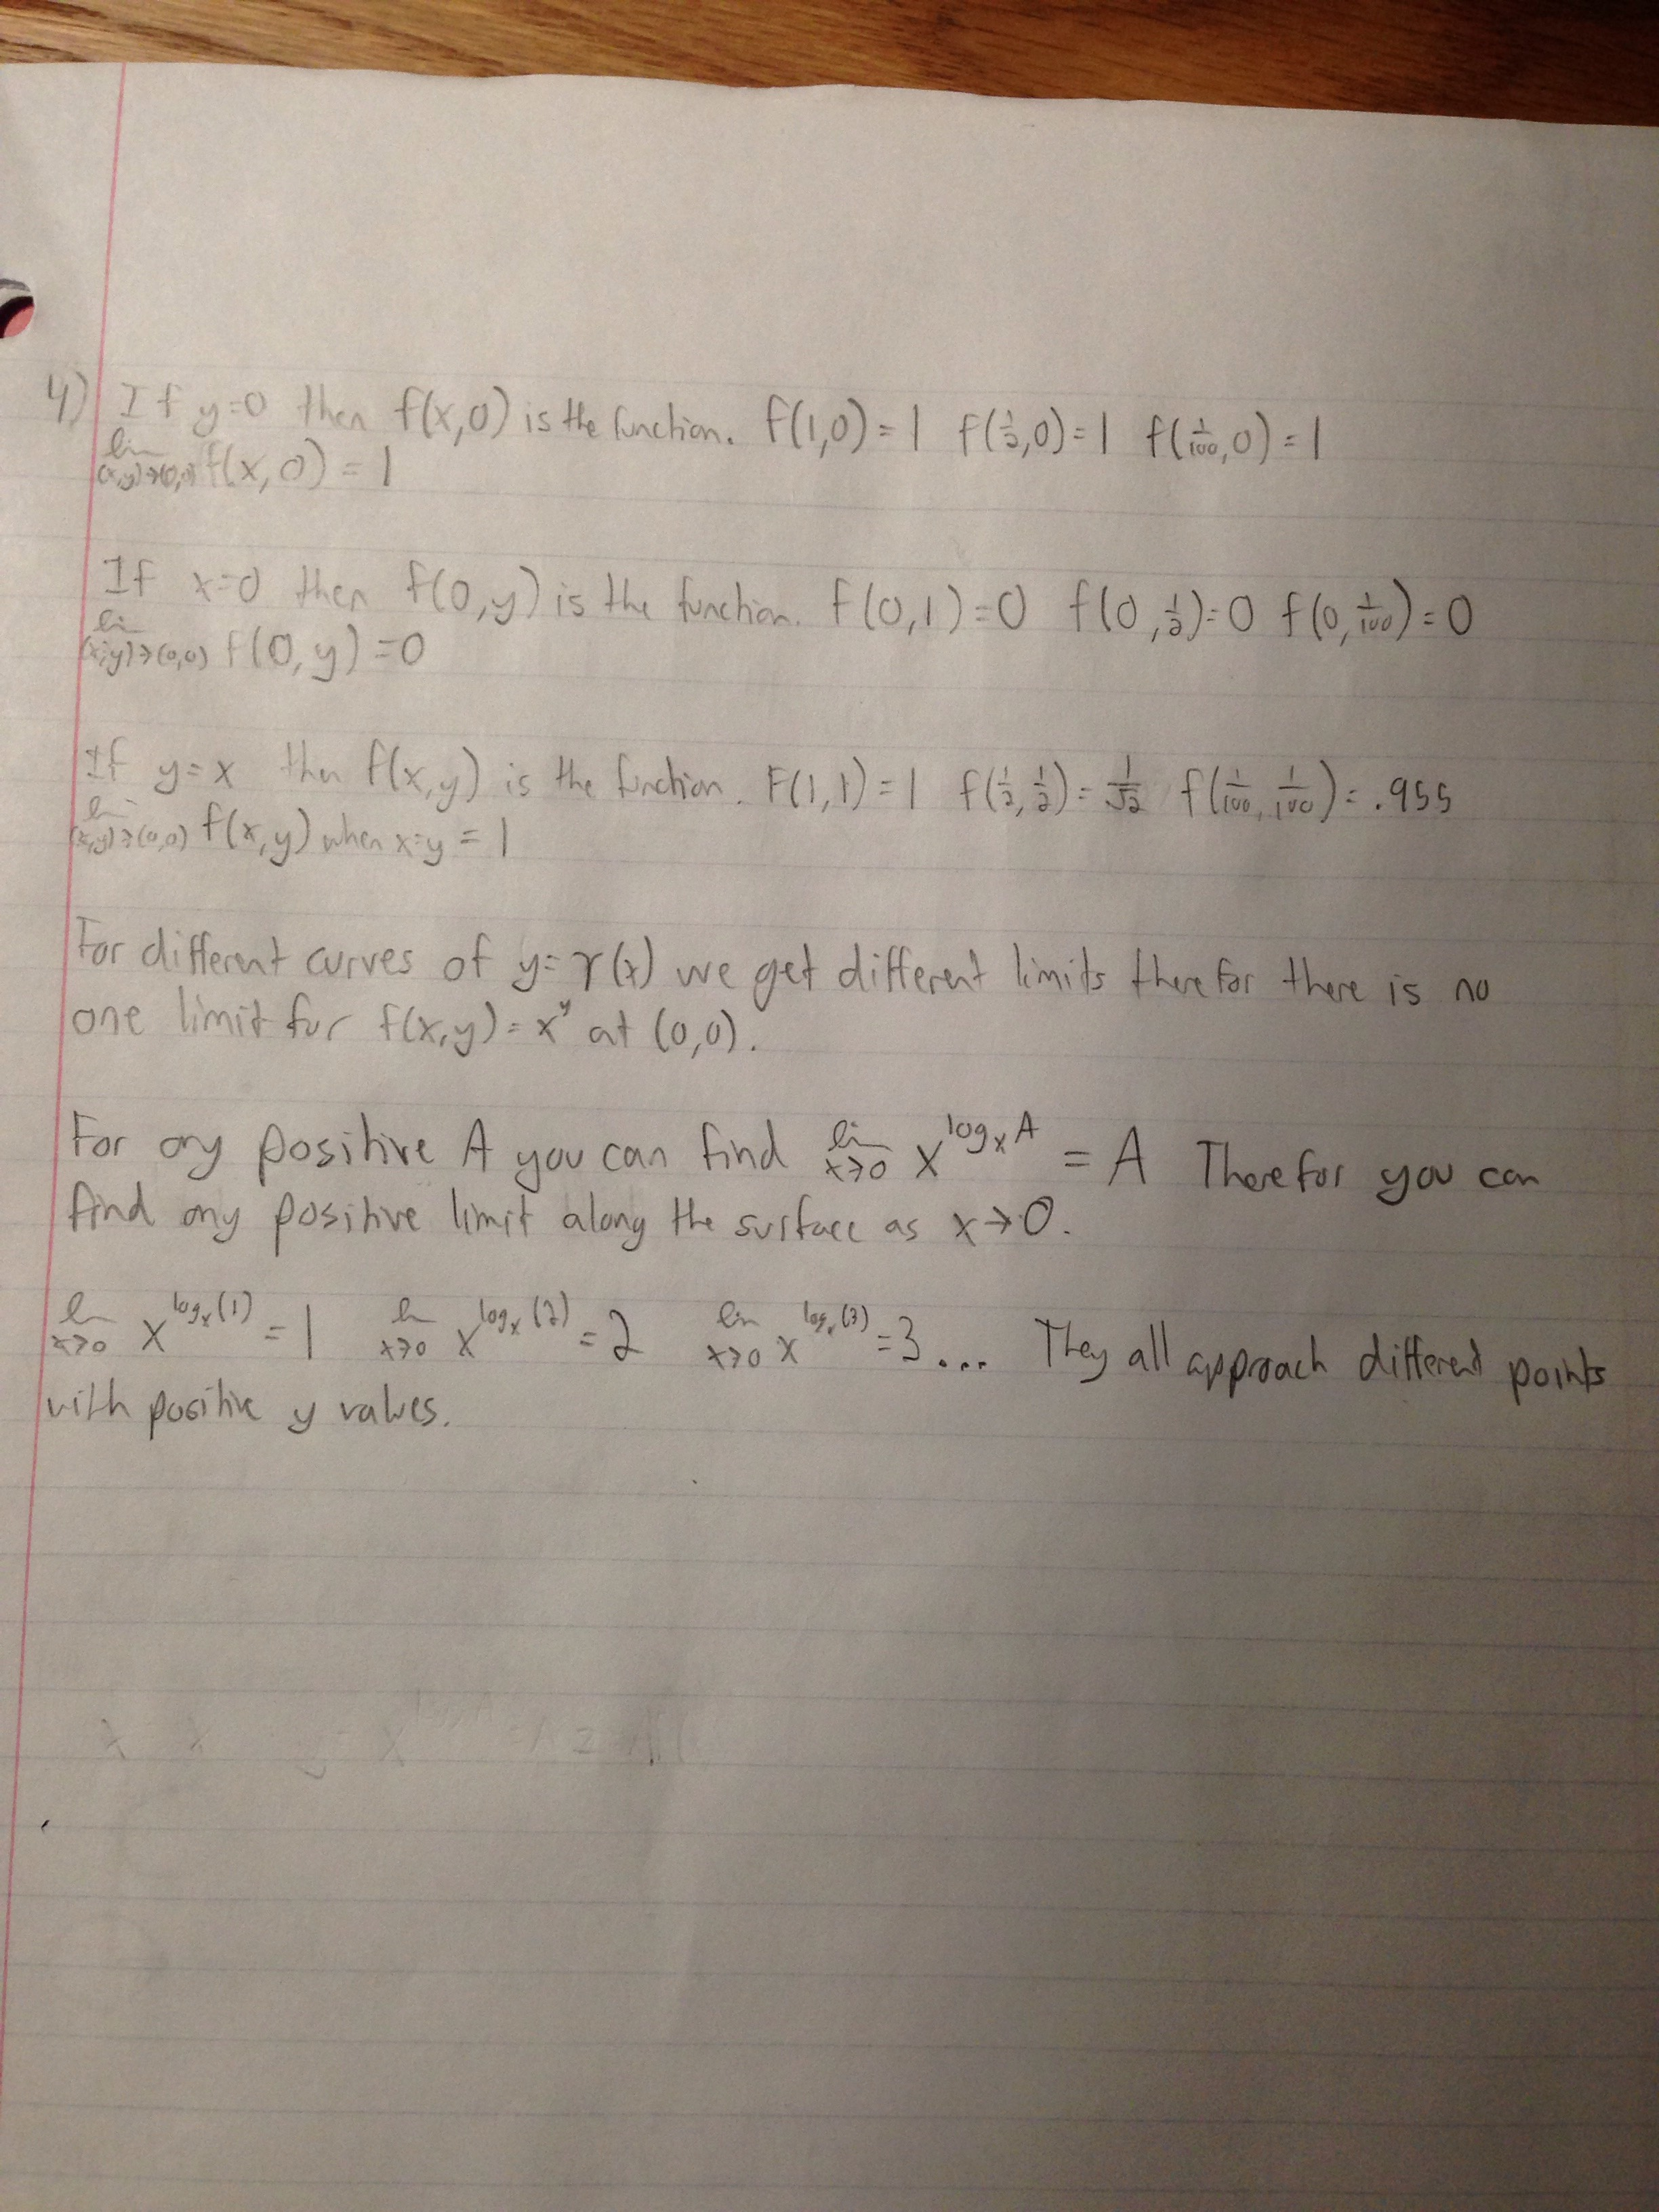
\includegraphics[width=\textwidth]{PartFour}
\end{figure}

\end{document}